\chapter{The Brain}
Amongst the algorithms for choosing the moves in turn-based games, we chose the \textit{alpha-beta pruning} algorithm.
It is a well known algorithm for turn based games, and can be thinked of as an evolution of the basic minimax algorithm, in fact it aims to reduce the number of nodes that are evaluated during the search.

We will discuss the plain minimax algorithm, then the alpha-beta pruning one, and finally the way we used it in our specific case.

\section{Minimax} \label{sec:minimax}
\textit{Minimax} is an algorithm for making decisions.
The hipothesis is that of a 2 player zero-sum game, where the outcome goes from -V to V.

One of the player tries to maximize the outcome, while the other tries to minimize it.
For readability sake, we will refer to the two players as to \textbf{Max} and \textbf{Min}.

\textbf{Max} and \textbf{Min} alternate in choosing a move, so each turn consists into two choices, each of which is called a ``ply''.
At each level of the search, the active player watches the outcome associated with each of the options he has, and chooses the one that maximizes his result.
Since the outcome for each of the options depends on the next choice of the other player, the actual choice also minimizes the opponent's result.
This is why the name ``minimax''.\\

\begin{figure}[htbp]
  \centering
    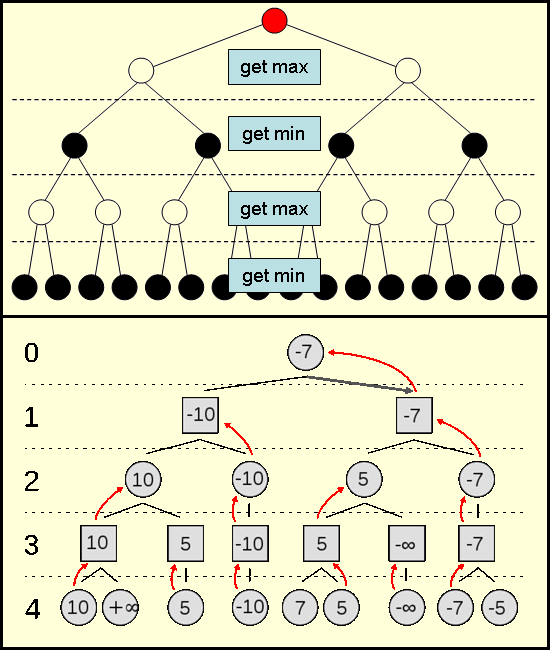
\includegraphics[width=0.5\textwidth]{images/minimax.png}
  \caption{Minimax choosing schema and a simple case example.}
\end{figure}

Of course, when the depth of the tree becomes too high to compute the actual outcome of a choice, we need to use some heuristics. Moreover, this algorithm assumes that the opponent plays with a ``perfect'' strategy, that is reasonable in normal turn-based games, but has some interesting effects when players choose more than a move each time (see chapter \ref{cap:results} for more on this).

\section{Alpha-Beta pruning}
As seen in section \ref{sec:minimax}, the minimax algorithm expands the tree up to a certain level, evaluating all the leaf nodes and backpropagating informations.
While descending in new branches, it doesn't take into account the previously computed heuristic values.
The \textit{alpha-beta pruning} algorithm tries to reduce the number of explored nodes, pruning branches when they are doomed to not be chosen.

Basically, when the algorithm explores a child node, keeps in memory the value of the best alternative's value for the \textbf{Max} and \textbf{Min} players (respectively alpha and beta), taking into account their turns succession.
If the explored child's value turns out to be too good for the active player (the player associated with that search level), that is it is better than the value that the opponent can force the active player to obtain making another decision in a preceding level, the remaining children won't be explored.\\
\\
The pseudo-code will clarify:\\
{\footnotesize
\lstset{language=C}
\begin{lstlisting}
  function alphabeta(node, level, search_depth, alpha, beta,
                     				maximizing)
  {
    if level==search		// this is a leaf node
    	return the heuristic value of the node
    
    if maximizing		// MAX player
    	for each child of node
        	alpha = max(alpha, alphabeta(child, level+1,
                			search_depth, alpha,
                        		beta, !maximizing)
                           )
                if beta <= alpha
                	break	// Beta cut-off
        return alpha
        
    else			// MIN player
    	for each child of node
        	beta = min(alpha, alphabeta(child, level+1,
                			search_depth, alpha,
                        		beta, !maximizing)
                           )
                if beta <= alpha
                	break	// Alpha cut-off
        return beta
  }
  
  -- first call:
  alphabeta(root, 0, search_depth, -infinite, +infinite, true)
\end{lstlisting}
}

\begin{figure}[htbp] \label{fig:alphabeta_example}
  \centering
    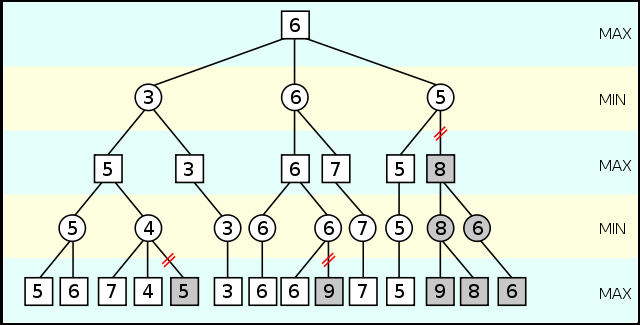
\includegraphics[width=0.5\textwidth]{images/alphabeta_pruning.png}
  \caption{Alpha-Beta Pruning use example. The darker nodes are not evaluated at all.}
\end{figure}

In figure \ref{fig:alphabeta_example} you can see a simple application of the alphabeta pruning algorithm. Notice that the algorithm, in some cases, prunes big portions of the tree. In the example given it may be a little advantage, but when the depth search and the branching factor grow this may lead to a huge resources saving.
